% Created 2015-06-20 Sáb 13:13
\documentclass[11pt]{article}
\usepackage[utf8]{inputenc}
\usepackage[T1]{fontenc}
\usepackage{fixltx2e}
\usepackage{graphicx}
\usepackage{longtable}
\usepackage{float}
\usepackage{wrapfig}
\usepackage{rotating}
\usepackage[normalem]{ulem}
\usepackage{amsmath}
\usepackage{textcomp}
\usepackage{marvosym}
\usepackage{wasysym}
\usepackage{amssymb}
\usepackage{hyperref}
\tolerance=1000
\usepackage{minted}
\usemintedstyle{perldoc}
\usepackage{tikz}
\usetikzlibrary{decorations.markings}
\tikzstyle{vertex}=[circle, draw, inner sep=0pt, minimum size=7pt]
\newcommand{\vertex}{\node[vertex]}
\author{Alice Duarte Scarpa, Bruno Lucian Costa}
\date{2015-06-23}
\title{Exercício 8.19 (Tardos)}
\hypersetup{
  pdfkeywords={},
  pdfsubject={},
  pdfcreator={Emacs 24.4.1 (Org mode 8.2.10)}}
\begin{document}

\maketitle

\section{Enunciado}
\label{sec-1}

Um comboio de navios chega ao porto com um total de $n$ vasilhames
contendo tipos diferentes de materiais perigosos.
Na doca, estão $m$ caminhões, cada um com capacidade para até $k$
vasilhames.  Para cada um dos dois problemas, dê um algoritmo
polinomial ou prove NP-completude:


\begin{itemize}
\item Cada vasilhame só pode ser carregado com segurança em alguns
dos caminhões. Existe como estocar os $n$ vasilhames nos $m$
caminhões de modo que nenhum caminhão esteja sobrecarregado, e
todo vasilhame esteja num caminhão que o comporta com segurança?

\item Qualquer vasilhame pode ser colocado em qualquer caminhão,
mas alguns pares de vasilhames não podem ficar juntos num mesmo
caminhão. Existe como estocar os $n$ vasilhames nos $m$
caminhões de modo que nenhum caminhão esteja sobrecarregado e
que nenhum dos pares proibidos de vasilhames esteja no mesmo
caminhão?
\end{itemize}

\section{Item a}
\label{sec-2}

Uma solução força-bruta para esse problema seria:

\begin{itemize}
\item Extenda a lista de vasilhames com vasilhames vazios, até que ela
tenha tamanho  $mk$ (a capacidade total de todos os caminhões).
\item Para cada uma das $(mk)!$ ordenações da lista acima, considere que
os $k$ primeiros vão para o primeiro caminhão, os $k$ próximos para
o segundo e assim até o final da lista. Se cada vasilhame estiver em
um camihão que o comporta com segurança, retorne essa solução, se
não, tente com uma nova ordem.
\end{itemize}

Esse algoritmo faz $(mk)!$ iterações do loop principal no pior caso, cada
iteração tem custo $mk$ para conferir se é uma solução válida. Isso dá
uma complexidade total de $O(mk(mk)!)$

Esse é um algoritmo super-exponencial para o problema, mas isso não
significa que o problema é NP-completo. Na verdade, como veremos a
seguir, esse problema não é NP-completo pois aceita uma solução
polinomial usando fluxos.

\subsection{Solução com fluxos}
\label{sec-2-1}

Podemos transformar esse problemas em um problema de encontrar o fluxo
máximo de um grafo usando a seguinte construção:

\begin{itemize}
\item Criamos um vértice $s$ representando a fonte e um vértice $t$
  representando o dreno

\item Para cada vasilhame $v_i \in v_1, v_2, \ldots, v_n$ criamos um
vértice $v_i$ e uma aresta $(s, v_i)$ capacidade 1

\item Para cada caminhão $C_i \in C_1, C_2, \ldots, C_m$ criamos um
vértice $C_i$. Se o vasilhame $v_j$ puder ser transportado com
segurança no caminhão $C_i$ criamos uma aresta $(v_j, C_i)$ de
capacidade 1. Para cada caminhão criamos também uma aresta $(C_i, t)$
de capacidade $k$.
\end{itemize}

Dessa forma, existe uma configuração possível de caminhões se e
somente se (TODO: provar) o fluxo máximo tem valor $m$.

A figura abaixo ilustra a construção para o caso com 7 vasilhames e 2
caminhões de capacidade 4. Em que os vértices pares podem ir no
caminhão 1 e os ímpares no caminhão 2:

\[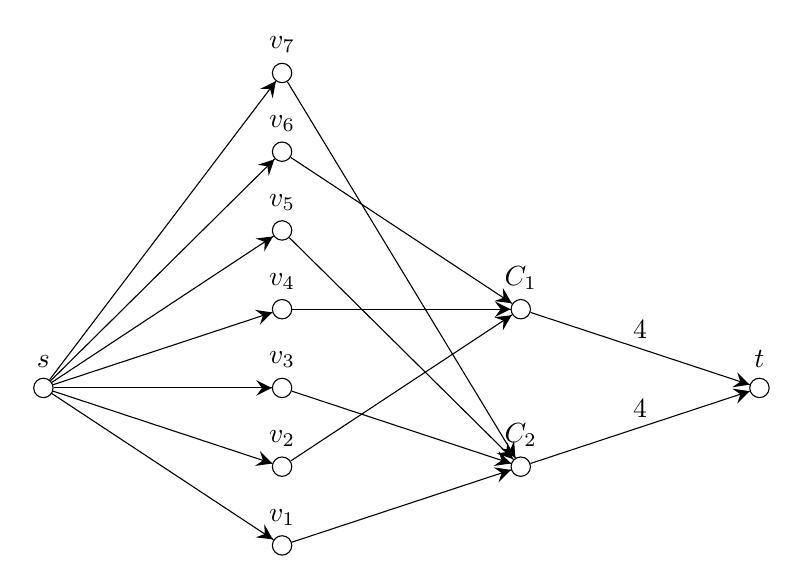
\begin{tikzpicture}[x=0.25\textwidth,
    every edge/.style={
        draw,
        postaction={decorate,
                    decoration={markings,mark=at position 1 with {\arrow[line width = 0.5mm]{stealth}}}
                   }
        }
]
\vertex (fonte) at (0,3) [label=above:$s$] {};
\vertex (v1) at (1,1) [label=above:$v_1$] {};
\vertex (v2) at (1,2) [label=above:$v_2$] {};
\vertex (v3) at (1,3) [label=above:$v_3$] {};
\vertex (v4) at (1,4) [label=above:$v_4$] {};
\vertex (v5) at (1,5) [label=above:$v_5$] {};
\vertex (v6) at (1,6) [label=above:$v_6$] {};
\vertex (v7) at (1,7) [label=above:$v_7$] {};
\vertex (C1) at (2,4) [label=above:$C_1$] {};
\vertex (C2) at (2,2) [label=above:$C_2$] {};
\vertex (dreno) at (3,3) [label=above:$t$] {};
\path
(fonte) edge (v1)
(fonte) edge (v2)
(fonte) edge (v3)
(fonte) edge (v4)
(fonte) edge (v5)
(fonte) edge (v6)
(fonte) edge (v7)
(v1) edge (C2)
(v2) edge (C1)
(v3) edge (C2)
(v4) edge (C1)
(v5) edge (C2)
(v6) edge (C1)
(v7) edge (C2)
(C1) edge node [above] {$4$} (dreno)
(C2) edge node [above] {$4$} (dreno)
;
\end{tikzpicture}\]

\subsubsection{Implementação}
\label{sec-2-1-1}

\subsubsection{Complexidade}
\label{sec-2-1-2}

\section{Item b}
\label{sec-3}
% Emacs 24.4.1 (Org mode 8.2.10)
\end{document}
